\documentclass[format=sigconf]{acmart}
\keywords{deep learning, neural network, biologically-motivated, equilibrium propagation, vanishing gradient, small-world, neuromorphic hardware}
\copyrightyear{2020}
\acmYear{2020}
%\setcopyright{licusgov}
\acmConference[ICONS 2020]{International Conference on Neuromorphic Systems 2020}{July 28--30, 2020}{Oak Ridge, TN, USA}
\acmBooktitle{International Conference on Neuromorphic Systems 2020 (ICONS 2020), July 28--30, 2020, Oak Ridge, TN, USA}
\acmPrice{}
\acmDOI{10.1145/3407197.3407618}
\acmISBN{978-1-4503-8851-1/20/07}


%\usepackage{cite}
\usepackage{natbib}
\usepackage{graphicx}
\usepackage{bm}
\usepackage{amsmath}
%\usepackage{amssymb}
%\usepackage{subcaption}
%\usepackage{mathtools}
%\usepackage[title]{appendix}
\usepackage[ruled,vlined]{algorithm2e}
\usepackage{hyperref}
%\usepackage{adjustbox}
%\usepackage[title]{appendix}
\usepackage[subtle]{savetrees}

\newcommand{\mtx}[1]{\bm{#1}}
\newcommand{\rms}[1]{<{#1}>}
\newcommand{\npar}{\\\indent}
\DeclareMathOperator*{\minimize}{minimize}

\title{Layer-skipping connections facilitate training of layered networks using equilibrium propagation.}
\author{Jimmy Gammell}
\author{Sae Woo Nam}
\author{Adam N. McCaughan}

\begin{CCSXML}
<ccs2012>
   <concept>
       <concept_id>10010147.10010257.10010293.10011809</concept_id>
       <concept_desc>Computing methodologies~Bio-inspired approaches</concept_desc>
       <concept_significance>500</concept_significance>
       </concept>
   <concept>
       <concept_id>10010147.10010257.10010293.10010294</concept_id>
       <concept_desc>Computing methodologies~Neural networks</concept_desc>
       <concept_significance>500</concept_significance>
       </concept>
%   <concept>
%       <concept_id>10010147.10010257.10010258.10010259</concept_id>
%       <concept_desc>Computing methodologies~Supervised learning</concept_desc>
%       <concept_significance>300</concept_significance>
%       </concept>
 </ccs2012>
\end{CCSXML}

\ccsdesc[500]{Computing methodologies~Bio-inspired approaches}
\ccsdesc[500]{Computing methodologies~Neural networks}
%\ccsdesc[300]{Computing methodologies~Supervised learning}

\begin{document}

\begin{abstract}

Equilibrium propagation is a learning framework that marks a step forward in the search for a biologically-plausible implementation of deep learning, and is appealing for implementation in neuromorphic analog hardware. However, previous implementations on layered networks encountered a vanishing gradient problem that has not yet been solved in a simple, biologically-plausible way. In this paper, we demonstrate that the vanishing gradient problem can be overcome by replacing some of a layered network's connections with random layer-skipping connections. This approach could be conveniently implemented in neuromorphic analog hardware, and is biologically-plausible.

\end{abstract}

\maketitle

\section{Introduction}

Equilibrium propagation \cite{scellier17} is a learning framework for energy-based networks such as the continuous Hopfield network \cite{hopfield1984}. It is appealing relative to backpropagation because it is more biologically-plausible, and as a side-effect could be implemented more-easily in neuromorphic analog hardware.
\npar
Implementation of equilibrium propagation in \cite{scellier17} was hindered by a vanishing gradient problem whereby networks with as few as 3 hidden layers trained slowly on MNIST \cite{mnist1998} - a serious issue given that network depth is critical to performance on difficult datasets \cite{simonyan2014, srivastava2015tvdn} and that convergence to a low error rate on MNIST is a low bar to meet. The problem was overcome in \cite{scellier17} by independently tuning a unique learning rate for each layer in the network; however, this approach is unappealing because (1) it introduces additional hyperparameters to tune, (2) it would be inconvenient to implement in neuromorphic analog hardware, and (3) it has not been observed in biological systems.
\npar
The purpose of this paper is to demonstrate that in this context the vanishing gradient problem can instead be solved by randomly replacing some of a layered network's connections with layer-skipping connections.
\footnote{This modification was inspired by small-world topology \cite{watts98}; however, we have not observed a strong correlation between network performance and common metrics of small-worldness (characteristic path length, clustering coefficient, small-world coefficient ).}
%\cite{humphries2008}).}
Through this modification we have achieved 0\% training error (out of 50,000 examples) and $\lesssim$2.5\% test error (out of 10,000 examples) on MNIST using a network with three hidden layers and no regularization term in its cost function. These error rates are comparable to those of other biologically-motivated networks \cite{bartunov2018} and are roughly the same as those of the layered network with unique, manually-tuned learning rates in \cite{scellier17}. Our method could be implemented with relative ease in any system with configurable connectivity. Layer-skipping connections have been observed in biological brains \cite{bullmore2009}, so the approach is biologically-plausible. Similar techniques have seen success in convolutional \cite{he2015, srivastava2015} and multilayer feedforward \cite{xiaohu2011, krishnan2019} networks. Our findings outlined in this paper suggest that layer-skipping connections are effective-enough to be appealing in contexts where simplicity and biological plausibility are important.

\section{Background and Theory}

\subsection{Equilibrium propagation}
\label{sec:eqp_formulation}

Similarly to backpropagation, equilibrium propagation \cite{scellier17} trains networks by approximating gradient descent on a cost function. Equilibrium propagation is applicable to any network with dynamics characterized by evolution to a fixed point of an associated energy function; our implementation is a recreation of that in \cite{scellier17}, which applies it to a continuous Hopfield network \cite{hopfield1984}. The mathematical formulation of the framework can be found in \cite{scellier17}.
\npar
A major reason backpropagation is not biologically-plausible is that to implement it, each neuron would need two distinct mechanisms for information transmission: one to transmit its activation to shallower neurons during the forward-propagation phase, and another to transmit error-correction information to deeper neurons during the backward-propagation phase \cite{bengio2015}. While this is easy in a digital computer that can oversee and manipulate an entire network, it would be cumbersome in hardware (biological or otherwise) consisting of many simple, independent computational nodes with limited ability to share information. In contrast, equilibrium propagation consists of a free phase (comparable to forward-propagation) and a weakly-clamped phase (comparable to backward-propagation) during which each neuron only needs to know the activations of neighboring neurons, so only one mechanism for information transmission is needed \cite{scellier17}. In a similar vein, to implement backpropagation each neuron would need mechanisms to compute both an activation value using activations of deeper neurons and error-correction information using that of shallower neurons. For equilibrium propagation a neuron would only need the ability to compute an activation given those of adjacent neurons \cite{scellier17}.

\subsection{Vanishing gradient problem}
\label{sec:vangrad}

Vanishing gradients are problematic because they reduce a network's rate of training. and could be difficult to represent in neuromorphic analog hardware due to limited bit depth.
\npar
The vanishing gradient problem is familiar in the context of conventional feedforward networks, where techniques such as the weight initialization scheme in \cite{glorot2010}, the use of activation functions with derivatives that do not lead to output saturation \cite{schmidhuber2015}, and batch normalization \cite{ioffe2015} have been effective at overcoming it. However, in the context of the networks trained in \cite{scellier17}, the vanishing gradient problem persists even when the former two techniques are used. To our knowledge batch normalization has not been used in the context of equilibrium propagation; however, it seems unlikely to be biologically-plausible.

\section{Implementation}
\label{sec:implementation}

\begin{figure}
  \centering
    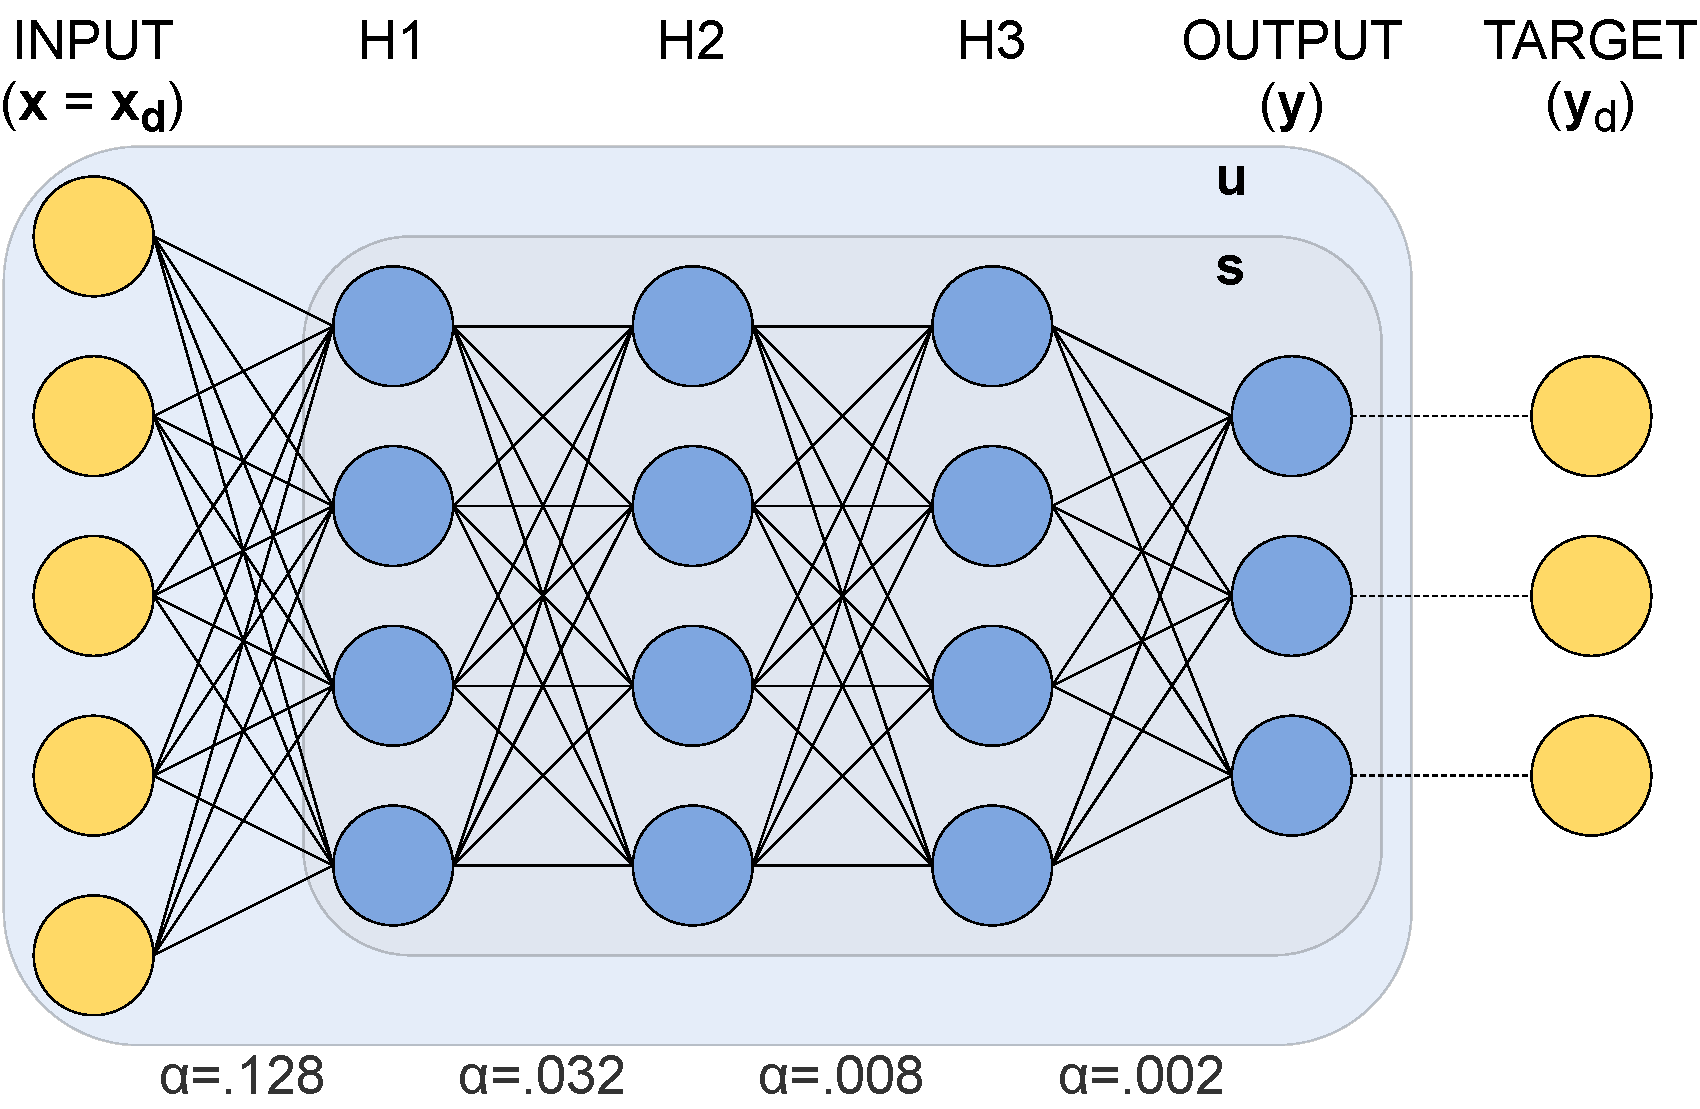
\includegraphics[width=\columnwidth]{figures/basic_topology_illustration.pdf}
    \caption{Topology of the layered network tested in \cite{scellier17}. All pairs of neurons in adjacent layers are connected. All connections are bidirectional. To compensate for the vanishing gradient problem, the learning rate is reduced by a factor of 4 each time distance from the output decreases by one layer.}
    \label{fig:top_basic}
\end{figure}
\hfill
\vspace{4mm}
\begin{figure}
	\centering
    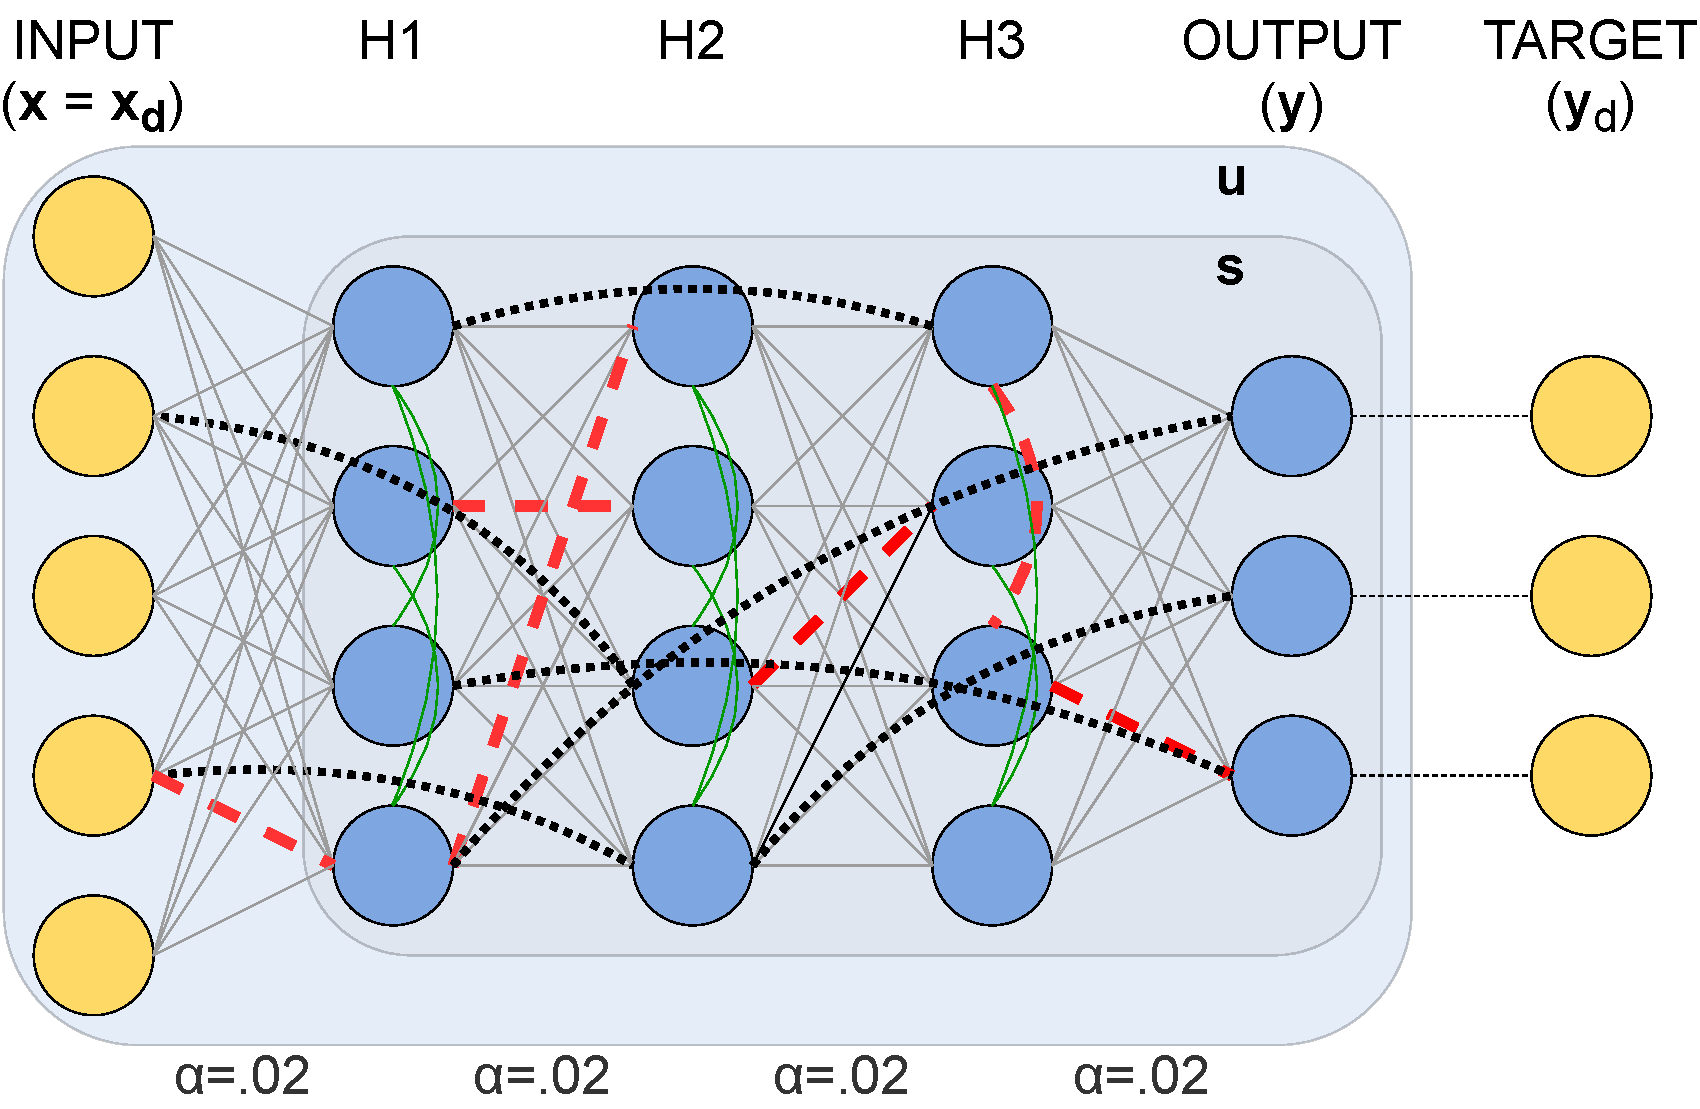
\includegraphics[width=\columnwidth]{figures/topology_changes_illustration.pdf}
     \caption{Our modifications to the topology of figure \ref{fig:top_basic} to avoid a vanishing gradient while using a global learning rate. Red dotted lines denote connections that have been removed, black dotted lines denote their replacements, and green solid lines denote added intralayer connections. All connections are bidirectional. This illustration shows a network with $p=8\%$.}

    \label{fig:top_sw}
\end{figure}

We recreated the equilibrium propagation implementation in \cite{scellier17} using the Pytorch library.
\footnote{\url{https://github.com/jgammell/Equilibrium_Propagation_mobile.git}}
 Like the networks in \cite{scellier17}, our networks are continuous Hopfield networks with a hardened sigmoid activation function $$\sigma(x)=\text{Max}\{0, \text{Min}\{x, 1\}\}$$ and squared-error cost function with no regularization term $$C=||\mtx{y}-\mtx{y}_d||_2^2,$$ where $\mtx{y}$ is the network's output and $\mtx{y}_d$ is the target output. Tests were run on MNIST \cite{mnist1998} grouped into batches of 20 examples, with the 50,000 training examples used for training and the 10,000 validation examples used for computing test errors.
\npar
We use two performance-enhancing techniques that were used in \cite{scellier17}: we randomize the sign of $\beta$ before training on each batch, which has a regularization effect, and we use persistent particles, where the state of the network after training on a given batch during epoch $n$ is used as the initial state for that batch during epoch $n+1$. Persistent particles reduce the computational resources needed to approximate the differential equation governing network evolution, and would be unnecessary in an analog implementation that can approximate the equation efficiently. Note that this technique leads to higher error rates early in training than would be present with a more-thorough approximation of the differential equation.

\subsection{Layered topology with per-layer rates}
\label{sec:basic_topology}

We recreated the 5-layer network evaluated in \cite{scellier17}. It has the standard layered topology shown in \ref{fig:top_basic}, and consists of a 784-neuron input layer, 3 500-neuron hidden layers and a 10-neuron output layer. Weights are initialized using the scheme from \cite{glorot2010}. As mentioned above, each layer has a unique learning rate; the rates are $\alpha_1=.128$, $\alpha_2=.032$, $\alpha_3=.008$ and $\alpha_4=.002$ where $\alpha_i$ is the learning rate for the connection weights between layers $i$ and $i+1$ and for the biases in layer $i$, and the input and output layers are denoted $i=1$ and $i=5$, respectively.

\subsection{Layered topology with global learning rate}
\label{sec:basic_topology_uniform}

To illustrate the vanishing gradient problem and provide a point of reference, we also tested the network in section \ref{sec:basic_topology} with a single global learning rate of .02.

\subsection{Our topology}
\label{sec:our_topology}


\begin{algorithm}
\KwIn{Layered network from section \ref{sec:basic_topology_uniform}}
\KwIn{Integer $n$, giving number of connections to replace}
\KwOut{A network with our modified topology}
\For{\upshape{hidden layer in network}}
{
	$\text{Add edge between each pair of neurons in layer}$
}
\For{$i\leftarrow 1$ \KwTo $n$}
{
	$\text{Randomly select pre-existing connection in network}$;\\
	$\text{Add connection between random unconnected pair of}$\\
	$\qquad\text{neurons in network}$;\\
	\tcp{Do not allow self connections}
	\tcp{Do not allow connections between two input neurons or between two output neurons}
	$\text{Remove pre-existing connection}$;
}
\Return{\upshape{modified network}}

\caption{Algorithm to produce our topology}
\label{alg:ourtop}
\end{algorithm}

To generate a network with our topology, we use algorithm \ref{alg:ourtop}. This topology is illustrated in figure \ref{fig:top_sw}. The above algorithm is approximately equivalent to the algorithm for generating a small-world network described in \citep{watts98} with $p=1-(\frac{N_o-1}{N_o})^n$ for $p\lesssim .2$, where $N_o$ is the number of connections in the network; to contextualize the number of replaced connections we will henceforth describe networks with our topology in terms of $p$ instead of $n$. We have seen good results with $p\approx 8\%$. We have seen similar results when connections are added to the network, rather than randomly replaced (algorithm \ref{alg:ourtop}, without removing pre-existing connections).
\npar
For these networks we use a global learning rate of .02 and, as in the networks from sections \ref{sec:basic_topology} and \ref{sec:basic_topology_uniform}, initialize connections between neurons in adjacent layers using the scheme from \cite{glorot2010}. For all other connections we draw initial weights from the uniform distribution $U[-.05, .05]$ where the value .05 was determined empirically to yield good results.

\section{Results}

\begin{figure}
  \centering
  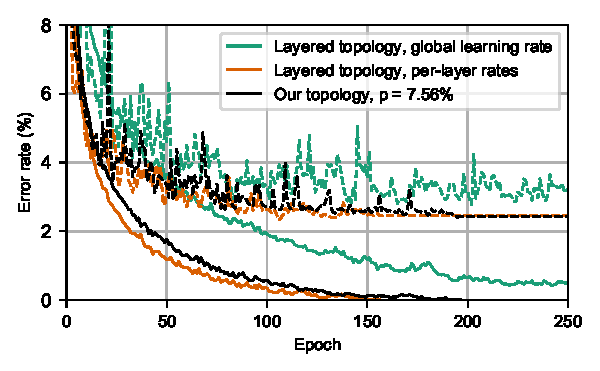
\includegraphics[width=\columnwidth]{figures/MNIST_network_comparison.pdf}
  \caption{Performance on MNIST of the networks in section \ref{sec:implementation}. Dashed lines show the test error and solid lines show the training error. In green is a layered network with a global learning rate (section \ref{sec:basic_topology_uniform}), in orange is a layered network with per-layer rates individually tuned to counter the vanishing gradient problem (section \ref{sec:basic_topology}), and in green is a network with our topology, $p=7.56\%$ (section \ref{sec:our_topology}). Observe that our topology is almost as effective as per-layer rates at countering the vanishing gradient problem that impedes training of the layered network with a global learning rate.}
  \label{fig:mnist_comparison}
\end{figure}

We compared the networks described in section \ref{sec:implementation} by observing their behavior while training on MNIST \cite{mnist1998}. All networks used $\epsilon=.5$, $\beta=1.0$, 500 free-phase iterations, 8 weakly-clamped-phase iterations, and were trained for 250 epochs.

\subsection{Network performance comparison}
\label{sec:network_performance}

Figure \ref{fig:mnist_comparison} illustrates that our network significantly outperforms one with a global learning rate, and achieves close to the same training and test error rates as one with unique learning rates, albeit after around 25\% more epochs. Both our network and the layered network with unique learning rates achieve approximately a 2.5\% test error and 0\% training error, whereas the layered network with a global learning rate has test and training error rates around .5\% higher than the other two networks; it is unclear whether it would converge given enough time, but it is clear that it is inferior.

\subsection{Training rates of individual pairs of layers}
\label{sec:mnist_perlayer}

\begin{figure}
  \centering
  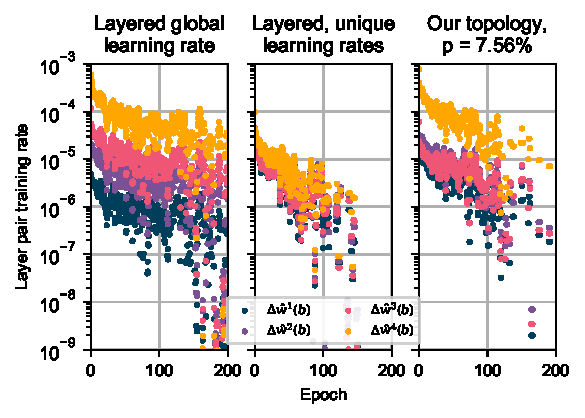
\includegraphics[width=\columnwidth]{figures/MNIST_individual_layers.pdf}
  \caption{Root-mean-square corrections to weights in different layers while training on MNIST, for the networks in section \ref{sec:implementation}. For clarity, values were subjected to an 11-point centered moving average. (left) A layered network with a single global learning rate (section \ref{sec:basic_topology_uniform}). (center) A layered network a unique, individually-tuned learning rate for each layer (section \ref{sec:basic_topology}).  (right) A network with our topology, $p = 7.56\%$ (section \ref{sec:our_topology}). Observe that the layered topology with a global learning rate has a vanishing gradient problem, which is almost completely solved by tuning an individual learning rate for each layer. Our topology improves the situation by making training uniform among the deeper layers, although the shallowest layer still trains more-quickly than the deeper layers.}  
  \label{fig:mnist_layers}
\end{figure}

To observe the extent of the vanishing gradient problem, for each network we tracked the root-mean-square correction to weights in each of its layers during training on MNIST \cite{mnist1998}. Figure \ref{fig:mnist_layers} shows an 11-point centered moving average of these values (without averaging the values are very volatile). It can be seen that for the layered network with a global learning rate, the magnitude of the correction to a typical neuron vanishes with depth relative to the output, with the shallowest weights training around 100 times faster than the deepest weights - this illustrates the vanishing gradient problem. The use of unique learning rates is very effective at making corrections uniform. Our topology with $p=7.56\%$ is effective at making deeper layers train in a uniform way, but the output layer still trains around 10 times faster than deeper layers; nonetheless, figure \ref{fig:mnist_comparison} suggests that this imperfect solution still yields a significant performance benefit.
\npar
The fast training of the output layer in the network with our topology is probably because no layer-skipping connections attach directly to the target output, so for any value of $p$ the shortest path between a deep neuron and the target layer is at least 2 connections long, whereas the path between an output neuron and the target layer is only 1 connection long.

\subsection{Effect of $p$}
%\label{sec:mnist_1epoch}
%
%\begin{figure}
%  \centering
%  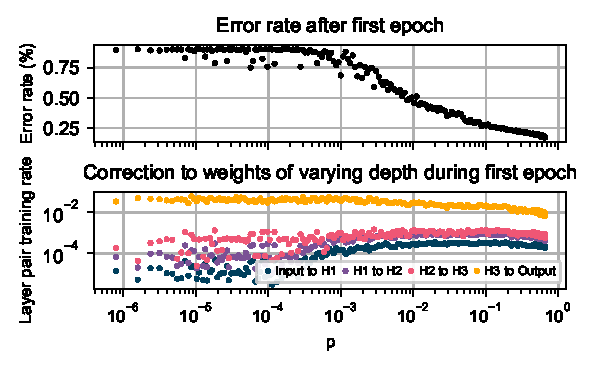
\includegraphics[width=\columnwidth]{figures/MNIST_one_epoch_performance.pdf}
%  \caption{Behavior of our network (section \ref{sec:our_topology}) with varying $p$, during the first epoch of training. (top) The training error after one epoch. (bottom) Root-mean-square correction to weights in different layers during the first epoch. Observe that as $p$ is increased, the error rate decreases and the root-mean-square corrections to each layer become more-uniform.}
%  \label{fig:mnist_1epoch}
%\end{figure}
%
We evaluated the behavior of our network during its first epoch of training on MNIST for varying $p$ and found that as $p$ increases, the error rate decreases and the root-mean-square corrections to each layer become more-uniform. We anticipate that generalization error will suffer for large $p$ as a network loses the benefits associated with a layered topology, but we did not train a large number of networks for long enough to observe such a trend. 
\npar
We noticed that networks with our topology and $p=0\%$ perform poorly relative to layered networks with a global learning rate; we believe this is due to a sub-optimal weight initialization. Networks with our topology seem less-sensitive to weight initialization than layered networks.

\section{Related work}
References \cite{lee2015, xie2003, pineda1987} describe other approaches to locally approximating the gradient of a cost function. References \cite{lillicrap2014, @crafton2019} explore the use of a random feedback matrix for backwards connections that is more biologically-plausible than identical forwards and backwards connections. Reference \cite{bartunov2018} explores the present state of biologically-motivated deep learning, and \cite{bengio2015} discusses the criteria a biologically-plausible network would need to satisfy. References \cite{shainline2019, davies2018, nahmias2013} discuss analog hardware that could potentially implement equilibrium propagation. References \cite{he2015, srivastava2015, xiaohu2011, krishnan2019} use layer-skipping connections for other types of networks and learning frameworks. References \cite{ioffe2015, glorot2010} give approaches to solving vanishing gradient problems.

\section{Directions for Future Research}

There are several directions in which future research could be taken:
\begin{itemize} 
\item Evaluating the effectiveness of this approach on hard datasets, such as CIFAR and ImageNet.
\item Evaluating the effect of $p$ on a network's test error.
\item Exploring the effectiveness of layer-skipping connections on deeper networks.
\item Exploring the effectiveness of a network when layer-skipping connections are used during training and removed afterwards.
\end{itemize}


\bibliographystyle{plain}

The U.S. Government is authorized to reproduce and distribute reprints for governmental purposes notwithstanding any copyright annotation thereon.


\bibliography{references}




\end{document}




